%versi 2 (8-10-2016) 
\chapter{Pendahuluan}
\label{chap:intro}
   
\section{Latar Belakang}
\label{sec:label}

% \textit{Rugby} adalah olahraga tim yang berasal dari abad ke-19 sebagai variasi dari permainan sepak bola. Dalam \textit{rugby}, tujuan dari olahraga ini adalah meletakkan bola di belakang garis \textit{try} lawan~\cite{rugby-wikipedia}. Olahraga ini dapat dimainkan dengan tangan dan juga tendangan, tetapi pemain hanya boleh melempar bola atau diserahkan ke belakang saat dibawa menggunakan tangan. \footnote{\url{https://www.sehataqua.co.id/apa-itu-olahraga-rugby/}}

Dikutip dari buku Olahraga Rugby (2010)~\cite{olahraga-rugby}, \textit{Rugby} merupakan olahraga yang berasal dari negara Inggris, di mana olahraga ini memiliki kemiripan dengan sepak bola. \textit{Rugby} berawal dari zaman Yunani Kuno, di mana seorang yang bernama William Webb Ellis melanggar aturan bermain bola pada tahun 1823 dengan membawa bola ke gawang lawan. Olahraga ini juga pertama kali diperkenalkan pada tahun 1986 pada zaman penjajahan, dan dihidupkan kembali pada tahun 2004 dengan bantuan negara lain seperti Australia dan Selandia Baru sehingga terbentuklah Indonesian Rugby Football Union (IRFU) yang bertujuan untuk mengembangkan olahraga ini.

% Persatuan Rugby Union Indonesia (PRUI) adalah organisasi yang bertanggung jawab atas pengelolaan dan pengembangan Rugby Union di Indonesia.\footnote{\url{https://www.asiarugby.com/unions/indonesia/}} PRUI ini memiliki tim nasional putra dan putri.\footnote{\url{https://rugbyindonesia.or.id/tentang/}} Tim nasional rugby union Indonesia mewakili Indonesia dalam rugby union dan dijuluki "Rhinos". Tim ini adalah anggota penuh World Rugby dan belum pernah bermain di Piala Dunia Rugby.\footnote{\url{https://en.wikipedia.org/wiki/Indonesia_national_rugby_union_team}} Rugby union di Indonesia adalah olahraga minor namun berkembang, yang telah ada selama beberapa dekade, dan mengalami fluktuasi dalam kesuksesannya.\footnote{\url{https://en.wikipedia.org/wiki/Rugby_union_in_Indonesia}} 

Dikutip dari Asia Rugby\footnote{\url{https://www.asiarugby.com/unions/indonesia/}}, Persatuan Rugby Union Indonesia atau yang biasa disingkat dengan PRUI merupakan Asosiasi Uni Rugbi Indonesia yang bertanggung jawab atas pengelolaan dan pengembangan Rugby Union di Indonesia yang dibangun. PRUI dibentuk pada tahun 2004 dan telah menjadi anggota penuh dari Komite Nasional Olahraga Indonesia atau yang biasa disingkat dengan KONI dan Komite Olimpiade Indonesia. PRUI juga memiliki banyak sejarah, seperti menjadi anggota penuh dari Asia Rugby dan World Rugby\footnote{\url{https://rugbyindonesia.or.id/tentang/}}. PRUI telah mengembangkan Rugby di berbagai sekolah di daerah Indonesia seperti Daerah Istimewa Yogyakarta, dan Jawa Barat. Pada tahun 2023, terdapat 35 klub rugby, 700 pemain terdaftar, 45 pelatih terdaftar, dan 23 wasit terdaftar di Indonesia \footnote{\url{https://rugbyindonesia.or.id/}}. Rugby Indonesia juga memiliki \textit{website}, di mana \textit{website} tersebut didirikan oleh PT. Dnartworks Komunikasi Visual untuk memberikan info seputar kegiatan olah raga \textit{rugby} yang berada di Indonesia. \textit{Website} ini didirikan menggunakan platform Wordpress.

Dikutip dari \footnote{\url{https://www.dicoding.com/blog/apa-itu-cms-wordpress/}}, Wordpress merupakan sebuah platform Content Management System (CMS) yang sangat populer untuk membangun \textit{website} dan blog. Diluncurkan pada tahun 2004 oleh Matt Mullenweg dan Mike Little, WordPress memungkinkan pengguna untuk membuat dan mengelola \textit{website} tanpa perlu memiliki pengetahuan dasar pemrograman. Content Management System (CMS) yang dibagun WordPress menggunakan bahasa pemrogramam PHP dan database MySQL. Dengan WordPress, pengguna baru dapat mengelola website tanpa perlu memahami teknis bahasa pemrograman, hal itu pun yang membuat para pemula dapat dengan mudah membuat website, bahkan dalam hitungan menit.

Dikutip dari GitHub Ionic~\cite{ionic-github}, Ionic Framework merupakan \textit{toolkit UI open-source} untuk membangun aplikasi modern, \textit{cross-platform} yang berkualitas tinggi dari satu kode sumber dengan JavaScript dan web. Ionic menyediakan alat dan layanan untuk mengembangkan aplikasi \textit{hybrid mobile, desktop}, dan \textit{progressive web} berdasarkan teknologi dan praktik pengembangan web modern, menggunakan teknologi web seperti CSS, HTML5, dan Sass. Ionic 7 merupakan versi \textit{stable release} terbaru dari Ionic, yang memperkenalkan cara kerja yang lebih efisien dengan kontrol formulir seperti \textit{Toggle} atau \textit{Input}. Komponen \textit{Item} dan Label tidak lagi diperlukan, dan setiap kontrol formulir menangani konten label secara langsung. Selain itu, fitur tertentu seperti teks bantuan atau mode pengisian \textit{input} telah dipindahkan dari \texttt{ion-item} ke kontrol formulir yang sesuai seperti \texttt{ion-input}, \texttt{ion-textarea}, dan \texttt{ion-select}. Perubahan ini mengurangi \textit{boilerplate} kode dengan menghilangkan persyaratan \texttt{ion-item} dan ion-label. Komponen Ionic Framework secara otomatis menyesuaikan tampilan dan nuansanya dengan platform di mana komponen tersebut dijalankan, memungkinkan gestur dan perilaku \textit{native} yang sama dengan yang biasa digunakan pengguna. Ionic memiliki lebih dari 100 komponen \textit{UI} yang telah dirancang sebelumnya, tipografi, dan tema dasar yang menyesuaikan dengan setiap platform. Ini dioptimalkan untuk \textit{mobile} dengan animasi yang diakselerasi oleh \textit{hardware}, \textit{lazy loading}, dan \textit{scrolling} 60FPS. Ionic CLI digunakan untuk membuat, membangun, dan menguji aplikasi serta memanfaatkan \textit{Live Reload, deployment}, dan dokumen~yang~baik.

% Capacitor adalah \textit{runtime native cross-platform} yang memudahkan pembuatan aplikasi \textit{mobile} yang performanya tinggi dan berjalan secara \textit{native} di iOS, Android, dan platform lainnya menggunakan \textit{web tooling modern}. Capacitor merupakan evolusi selanjutnya dari aplikasi \textit{hybrid}, yang menciptakan aplikasi \textit{Web Native} dengan pendekatan \textit{native container} modern untuk tim yang ingin membangun aplikasi \textit{web-first} tanpa mengorbankan akses penuh ke SDK \textit{native} ketika dibutuhkan. Capacitor menyediakan kumpulan API yang konsisten dan berfokus pada web yang memungkinkan aplikasi tetap dekat dengan standar web sebanyak mungkin, sambil mengakses fitur perangkat \textit{native} yang kaya pada platform yang mendukungnya. Capacitor dapat menambahkan fungsionalitas \textit{native} dengan mudah menggunakan \textit{Plugin} API untuk Swift di iOS, Java di Android, dan JavaScript untuk web. Capacitor 3.0 memiliki peningkatan kinerja, pengalaman untuk mengembangkan yang lebih baik, dan keterlibatan komunitas yang lebih besar. Capacitor dapat diintegrasikan dengan mudah ke dalam proyek JavaScript modern yang ada atau proyek Capacitor yang~baru.

Dikutip dari dokumentasi Capacitor~\cite{capacitor-docs}, Capacitor merupakan \textit{runtime native open source} yang dapat digunakan untuk membangun aplikasi Web Native. Capacitor memungkinkan pengembang untuk membangun aplikasi \textit{mobile} pada perangkat iOS dan Android. Selain itu, Capacitor juga memungkinkan pengembang untuk membangun aplikasi web progresif. Aplikasi yang dibangun akan menggunakan JavaScript, HTML, dan CSS. Capacitor juga menyediakan \textit{cross-platform} API yang dapat digunakan pada berbagai platform seperti iOS, Android, Web dengan satu kode sumber. Capacitor ini sendiri dikembangkan oleh tim Ionic, di mana tim ini jugalah yang mengembangkan \textit{framework} Ionic. Capacitor dirancang untuk menggantikan Apache Cordova, yang merupakan \textit{runtime} yang digunakan oleh Ionic sebelumnya. Capacitor ini juga memiliki beberapa keunggulan dibandingkan Apache Cordova, diantaranya adalah lebih ringan, lebih cepat, lebih modern, dan lebih fleksibel.

Dikutip dari dokumentasi RSS\footnote{\url{https://www.rssboard.org/rss-specification}}, RSS atau Really Simple Syndication adalah format sindikasi konten web yang merupakan dialek dari XML. Semua file RSS harus disesuaikan dengan spesifikasi XML 1.0 yang dipublikasikan oleh World Wide Web Consortium (W3C). Dokumen RSS terdiri dari elemen \texttt{<rss>} yang memiliki atribut wajib bernama version untuk menentukan versi RSS yang digunakan. Di bawah elemen \texttt{<rss>} terdapat elemen \texttt{<channel>} yang berisi informasi tentang saluran (metadata) dan isinya.

Pada sekitar tahun 2015, perusahaan PT. DNArtworks Komunikasi Visual membuat aplikasi Rugby Indonesia yang memanfaatkan Apache Cordova. Aplikasi tersebut memiliki: 
\begin{itemize}
    \item Halaman \textit{Latest News} yang diambil dari \url{https://rugbyindonesia.or.id/berita/} dengan memanfaatkan~protokol~RSS. {(Lihat gambar \ref{fig:rugby-halaman-label})}
    \item Halaman \textit{Fixture \& Results}, namun sekarang sudah tidak ada. {(Lihat gambar \ref{fig:rugby-halaman-label})}
    \item Halaman \textit{Teammate Photos} dengan fungsi:
    \begin{itemize}
        \item Pengguna dapat langsung mengambil foto dari aplikasi tersebut.
        \item Pengguna dapat langsung memberikan \textit{frame} terhadap foto tersebut.
        \item Pengguna dapat langsung mengunggah foto tersebut ke dalam galeri publik.
    \end{itemize}
    \item Halaman \textit{Rugby Clubs} yang memiliki fungsi di mana pengguna dapat melihat klub \textit{rugby} serta info dari klub tersebut pada tiap daerah. {(Lihat gambar \ref{fig:rugby-halaman-label})}
\end{itemize}

\begin{figure} [!h]
    \centering
    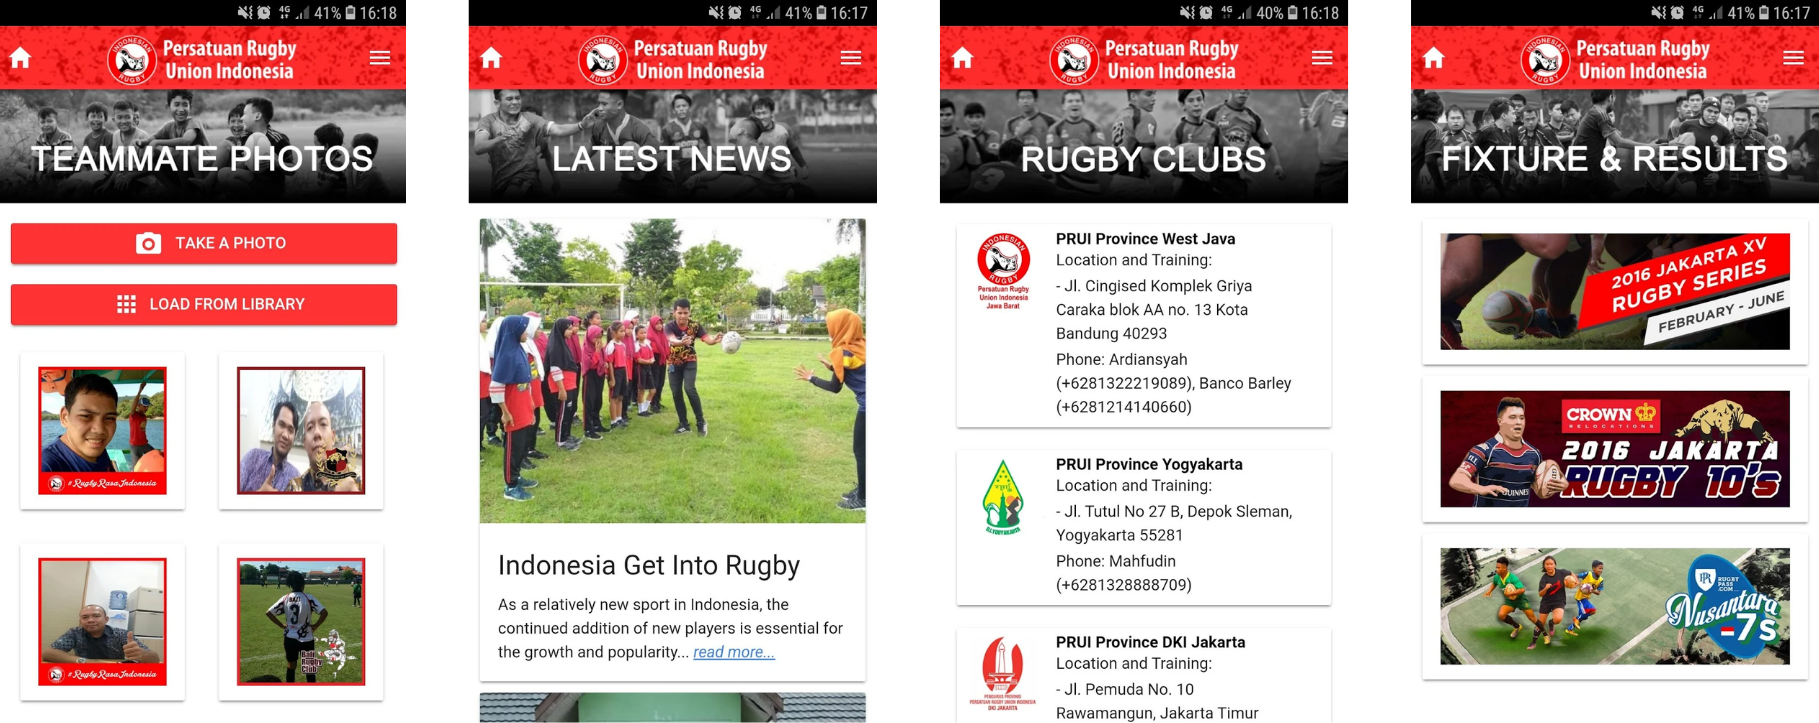
\includegraphics[scale=0.725]{Gambar/Rugby-Indonesia-App-UI.png}
    \caption[Halaman aplikasi Rugby Indonesia]{Halaman dari aplikasi Rugby Indonesia dari Google Play Store}
    \label{fig:rugby-halaman-label}
\end{figure}

Pada saat ini, aplikasi tersebut masih tersedia di Google Play Store\footnote{\url{https://play.google.com/store/apps/details?id=id.or.rugbyindonesia.androidapp\&hl=in}}, namun aplikasi tersebut tidak dapat dipasang pada perangkat Android saat ini dikarenakan \textit{website} \url{https://rugbyindonesia.or.id} sudah berubah dan juga Apache Cordova yang sudah tidak dapat digunakan kembali pada pengembangan aplikasi berbasis \textit{framework} Ionic dikarenakan Ionic sendiri telah mengembangkan Native Capacitor sehingga Ionic dapat melepas ketergantungannya pada Angular dan Cordova~\footnote{\url{https://ionic.io/blog/ionic-isnt-cordova-anymore}}. Maka dari itu pada skripsi ini, akan dibuat ulang sebuah perangkat lunak Rugby Indonesia yang terbaru, sehingga perangkat lunak tersebut dapat \textit{compatible} dengan perangkat android saat ini dengan memanfaatkan \textit{backend} aplikasi yang sudah dibuat menggunakan Wordpress dan juga protokol RSS untuk melakukan komunikasi antar \textit{backend} dan juga \textit{frontend}. Perangkat lunak ini juga akan memanfaatkan Capacitor bawaan dari Ionic yang berfungsi untuk membangun antarmuka secara \textit{native}.

Perangkat lunak ini akan dibuat dengan memanfaatkan bantuan {\it framework} Ionic 7 dan Native Capacitor dengan memiliki:
\begin{itemize}
    \item Halaman \textit{Latest News}, di mana pengguna dapat melihat berita terbaru dari Rugby Indonesia.
    \item Halaman \textit{Teammate Photos} di mana pengguna dapat mengambil foto dan langsung mengunggahnya ke dalam halaman \textit{teammate photos}.
    \item Halaman \textit{About Us} di mana pengguna dapat melihat tentang Rugby Indonesia.
\end{itemize}


% Bagian ini akan diisi dengan apa yang melatarbelakangi pembuatan template skripsi ini.
% Termasuk juga masalah-masalah yang akan dihadapi untuk membuatnya, termasuk kurangnya kemampuan penguasaan \LaTeX{} sehingga template ini dibuat dengan mengandalkan berbagai contoh yang tersebar di dunia maya, yang digabung-gabung menjadi satu jua.
% Bagian lain juga akan dilengkapi, untuk sementara diisi dengan lorem ipsum versi bahasa inggris.

% \dtext{5-10}

\section{Rumusan Masalah}
\label{sec:rumusan}
Rumusan masalah yang akan dibahas pada tugas akhir ini adalah sebagai berikut:
\begin{enumerate}
    \item Bagaimana membangun ulang serta mengembangkan perangkat lunak Rugby Indonesia dengan memanfaatkan \textit{framework} Ionic 7?
    \item Bagaimana membangun ulang serta mengembangkan perangkat lunak Rugby Indonesia dengan memanfaatkan Capacitor Native?
\end{enumerate}
% Bagian ini akan diisi dengan penajaman dari masalah-masalah yang sudah diidentifikasi di bagian sebelumnya. 

% \dtext{6}

\section{Tujuan}
\label{sec:tujuan}
Tujuan yang ingin dicapai pada penulisan tugas akhir ini yaitu:
\begin{enumerate}
    \item Pembuatan ulang aplikasi Rugby Indonesia yang sudah memanfaatkan \textit{framework} dari Ionic terbaru yaitu Ionic 7.
    \item Pembuatan ulang aplikasi Rugby Indonesia yang sudah memanfaatkan Native Capacitor.
\end{enumerate}
% Akan dipaparkan secara lebih terperinci dan tersturkur apa yang menjadi tujuan pembuatan template skripsi ini

% \dtext{7}

\section{Batasan Masalah}
\label{sec:batasan}
Batasan masalah yang terdapat pada pengerjaan tugas akhir ini yaitu:
\begin{enumerate}
    \item Perangkat lunak ini dibuat untuk perangkat Android saja, tidak untuk iOS. Sehingga pengujian dari perangkat lunak ini hanya dilakukan pada platform berbasis android saja. Perangkat lunak ini hanya dibuat untuk perangkat lunak android dikarenakan peneliti tidak memiliki perangkat lunak yang menggunakan sistem operasi iOS.
    \item Pengguna hanya bisa mengunggah foto dan melihat foto unggahan dari pengguna lain, pengguna tidak dapat menghapus ataupun mengubah foto tersebut. Hal ini dikarenakan pada aplikasi sebelumnya, pengguna hanya dapat melakukan hal tersebut.
\end{enumerate}
% Untuk mempermudah pembuatan template ini, tentu ada hal-hal yang harus dibatasi, misalnya saja bahwa template ini bukan berupa style \LaTeX{} pada umumnya (dengan alasannya karena belum mampu jika diminta membuat seperti itu)

% \dtext{8}

\section{Metodologi}
\label{sec:metlit}
Langkah-langkah yang dilakukan dalam pengerjaan tugas akhir ini yaitu:
\begin{enumerate}
    \item Melakukan studi literatur serta mendalami ReactJS sebagai salah satu perpustakaan JavaScript untuk membangun tampilan antar muka.
    \item Melakukan studi literatur mengenai \textit{framework} Ionic 7 dan juga Capacitor yang terdapat pada Ionic Native.
    \item Melakukan analisis terhadap perangkat lunak yang ada dan melakukan perancangan terhadap perangkat lunak yang akan dibuat.
    \item Membangun aplikasi Rugby Indonesia yang sudah menggunakan \textit{framework} Ionic 7 serta Capacitor.
    \item Melakukan pengujian dan eksperimen.
    \item Menulis dokumen tugas akhir.
\end{enumerate}
% Tentunya akan diisi dengan metodologi yang serius sehingga templatenya terkesan lebih serius.

% \dtext{9}

% \section{Sistematika Pembahasan}
% \label{sec:sispem}
% Penulisan setiap bab pada dokumen tugas akhir ini yaitu:
% \begin{enumerate}
%     \item Bab Pendahuluan
    
%     Bab 1 berisi latar belakang, rumusan masalah, tujuan, batasan masalah, metodologi, dan sistematika pembahasan yang digunakan untuk menyusun skripsi ini.

%     \item Bab Dasar Teori
    
%     Bab 2 berisi teori-teori yang digunakan dalam pembuatan skripsi ini. Teori-teori tersebut yaitu Rugby Union Indonesia, ReactJS, Ionic 7 Framework, Capacitor, UI Components.

%     \item Bab Analisis
    
%     Bab 3 berisi analisis yang dilakukan pada skripsi ini, meliputi analisis sistem kini, analisis kebutuhan aplikasi Rugby Indonesia yang akan dibangun, serta permasalahan pembangunan sistem usulan.

%     \item Bab Perancangan
    
%     Bab 4 berisi perancangan aplikasi meliputi perancangan kelas beserta dengan diagram kelas, deskripsi kelas dan fungsinya, serta perancangan struktur HTML.

%     \item Bab Implementasi dan Pengujian
    
%     Bab 5 berisi implementasi dan pengujian aplikasi meliputi lingkungan implementasi, hasil implementasi, pengujian fungsional, dan pengujian eksperimental.
    
%     \item Bab Kesimpulan dan Saran
    
%     Bab 6 berisi kesimpulan dari hasil pembangunan aplikasi ini dan saran untuk pengembangan selanjutnya.
% \end{enumerate}
% Rencananya Bab 2 akan berisi petunjuk penggunaan template dan dasar-dasar \LaTeX.
% Mungkin bab 3,4,5 dapt diisi oleh ketiga jurusan, misalnya peraturan dasar skripsi atau pedoman penulisan, tentu jika berkenan.
% Bab 6 akan diisi dengan kesimpulan, bahwa membuat template ini ternyata sungguh menghabiskan banyak waktu.

% \dtext{10}